\section{Our Method}
\label{sec:Meth}


\subsection{System Overview}
\label{subsection:overview}

\begin{figure}[!htq]
	\centering
	\includegraphics[width=3.4in]{figure/pipeline.eps}
	\caption{An overview of our layout estimation algorithm pipeline. First we adopt a multi-scale CNN achitecture to predict geometric information from RGB image, including depth and normals. Then we encode abovementioned information into FCNN , which help to accurately estimate the layout. Optimization framwork based on perspective projection restriction is adopted to generate final precise layout estimates.}
	\label{fig:pipeline}
\end{figure}

Under the Manhattan world assumption, a room layout is represented as cube having at most five walls (Left, Front, Right, Ceiling, Ground) visible in the image. 
%
Given an RGB image $I$ with \cxj{arbitrary?} size $w\times h$, our algorithm generates a room layout $\vb{L}$ consisting of a surface label for each pixel $L_{ij}\in $ $\{$left wall, front wall, right wall, ceiling, ground$\}$. 
Fig. \ref{fig:pipeline} shows our algorithm pipeline. 
%%step 1
Different from \cite{dasgupta2016delay}, we first estimate the depth depth $D_{I}$ and normal map $N_{I}$ from the input color image to generate \emph{geometric hints} using a multi-scale convolutional architecture~\cite{eigen2015predicting}, as described in Sec.~\ref{sec:depth_normal}.
%step 2
Integrating the original RGB image, the estimated depth and the normal map, a fully convolutional network is used to predict five surface maps, each of which describes the belief for each specific layout surface. Details will be described in Sec.~\ref{sec:surfacelabel}.
%step 3: optimization
To generate more clear and straight boundaries in the final layout, an optimization step is adopted to \cxj{what does this optimzation do?}, as described in Sec.~\ref{sec:optimization}.


\cxj{several questions here }

\begin{enumerate}
	\item \textbf{input image size}: as claimed in \cite{ren2016three}, the receptive field of VGG16 is 404x404, why do we use $321\times 321$?

\end{enumerate}
 

\comments{
The coarse layout estimation about semantic layout surfaces for a single RGB image, are predicted by fully convolutional neural network with geometric information emmbeded, including depth and normal information. These geometric information are estimated from source RGB image by a multi-scale convolutional architecture\cite{eigen2015predicting}. This will be decribied in Sec. \ref{subsection:CNN}. Then based on optimization framwork proposed in \cite{dasgupta2016delay}, which mainly uses perspective projection constraints, we can obtain final precise layout estimation results.
%
}
\cxj{Figure 3 is very similar with \cite{dasgupta2016delay}..}
 


\subsection{Geometric Fusion FCNN for Coarse Layout Estimation}
\label{sec:depth_normal}

We use the multi-scale convolutional network proposed in \cite{eigen2015predicting} to estimate the depth and normal map from a single RGB image, as Figure~\ref{fig:depthandnormal} shows. 
%
\cxj{More analysis on the results of depth map and normal map.}


\begin{figure}
	\centering
	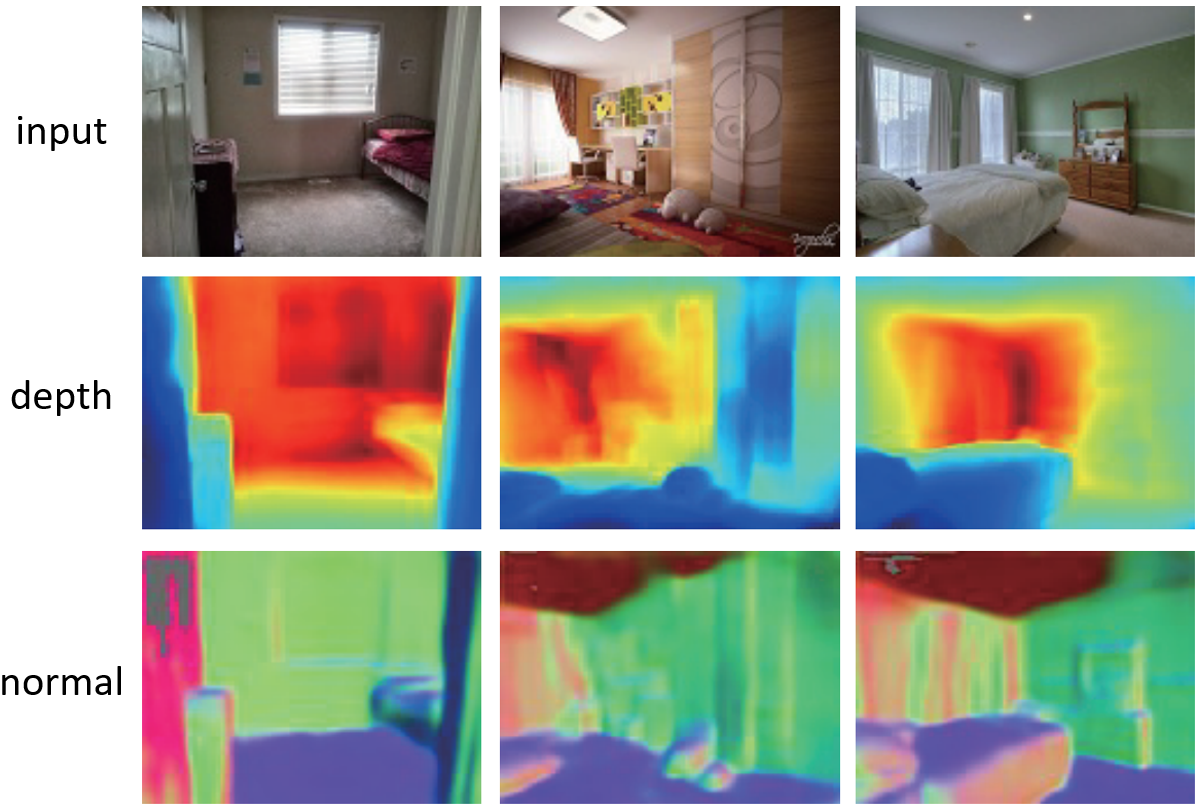
\includegraphics[width=\columnwidth]{figure/geometricinfo1.png}
	\caption{Estimation of depth and normal from a single RGB image using the multi-task FCN in \cite{eigen2015predicting}.}
	\label{fig:depthandnormal}
\end{figure}

\mdf{Though the predicted depth and normal are not accurate}, they provide valuable 3D information for high-level structure estimation, especially in cluttered scenes.
%
Normals can serve as clues tending to merge big planes together, with interference factors like clutter, textures and illumination eliminated to varying degrees. 
%
These mid-level geometric information can be used to adapt and improve performance for layout estimation compared to using RGB only. 



\subsection{Surface Label Prediction using MFCN}
\label{sec:surfacelabel}
%
In previous work, \cite{dasgupta2016delay,ren2016coarse} achieved to use fully convolutional neural network(FCNN) or multi-task fully convolutional neural network~(MFCNN) to predict coarse semantic layout surfaces and layout edges. 
%
However, due to much clutter, complex textures and illumination variations existed, semantic surfaces like walls are visually separated in to pieces, making whole surfaces difficult to aggregate together. 
%
Fig.~\ref{fig:fcn-comparison}(b) shows layout estimation results using FCNN architecture for prediction using a general FCN widely used in previous methods \cite{dasgupta2016delay,ren2016coarse}. 
Under the comparison between the predicted results and the ground truth, we can see that due to the environmental effect of indoor scenes, layout results estimated from FCNN are not reliable. 
When there exits clutter right on the boundaries, such critical clues are partially or entirely excluded, and thus we can not tell location of each plane precisely. 
Moreover, an entire plane may be predicted separately into pieces due to clutter lay in the plane.

\textbf{Network Architecture}
\cxj{Explain the network architecture.}

Given the input RGB image and the estimated geometric information including depth and normal, there are several possible ways to integrate them in a network to predict the surface labels. We introduce two architectures here.
We also resize them to $321 \time 321$ as input to the following FCN. 

The first way is treading the depth and normal map as four additional channels associated with the input RGB image. Given the seven-channel input (3 channels from RGB, 1 channel from depths and 3 channels from normals), we train a \mdf{VGG16 FCN} to predict the five belief maps for the five surfaces in a room. The network architecture is shown in Fig.~\ref{fig:fcn-multi-channel}. This architecture is named as FCN-MC in this paper. 
%
However, it is intuitively seen that different channels have a wide range of variance and they probably can not be directly fused at the beginning convolutional layers. 

\begin{figure}
	\centering
	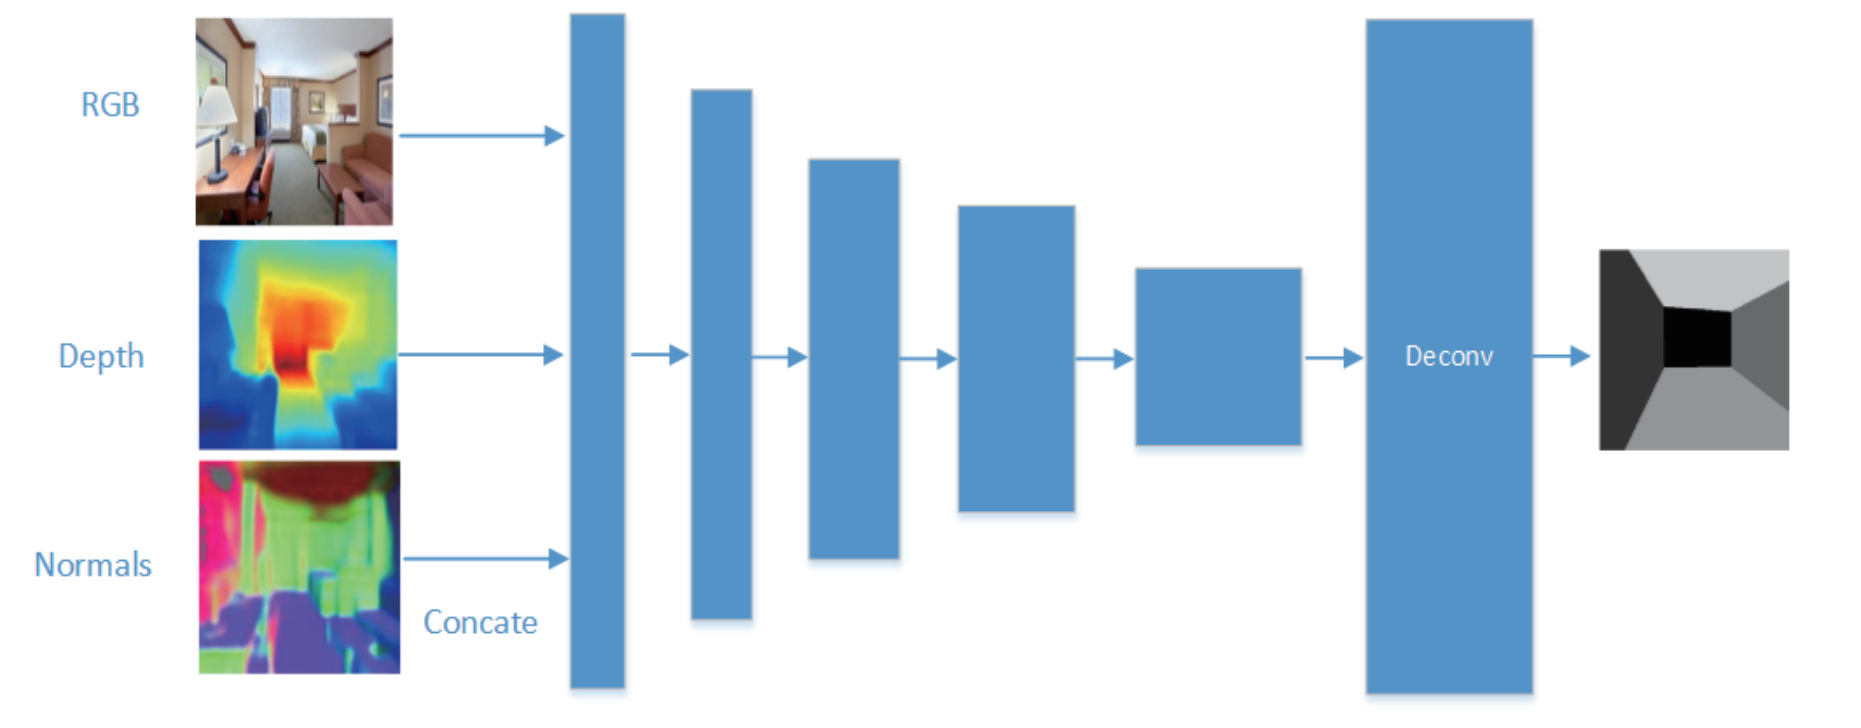
\includegraphics[width=\columnwidth]{figure/fcn-multi-channel.png}
	\caption{A simple network architecture taking the RGB, depth and normal together as input to a VGG16 FCN. \cxj{add more details of each layer.}}
	\label{fig:fcn-multi-channel}
\end{figure}

The second way to integrate them is to later fuse the features that are extracted from different channels separately with a number of convolutional layers. 
This network is named as FCN-GF (geometric fusion), whose architecture is shown in Fig.~\ref{fig:fcn-geometric-fusion}.
  
\begin{figure}
	\centering
	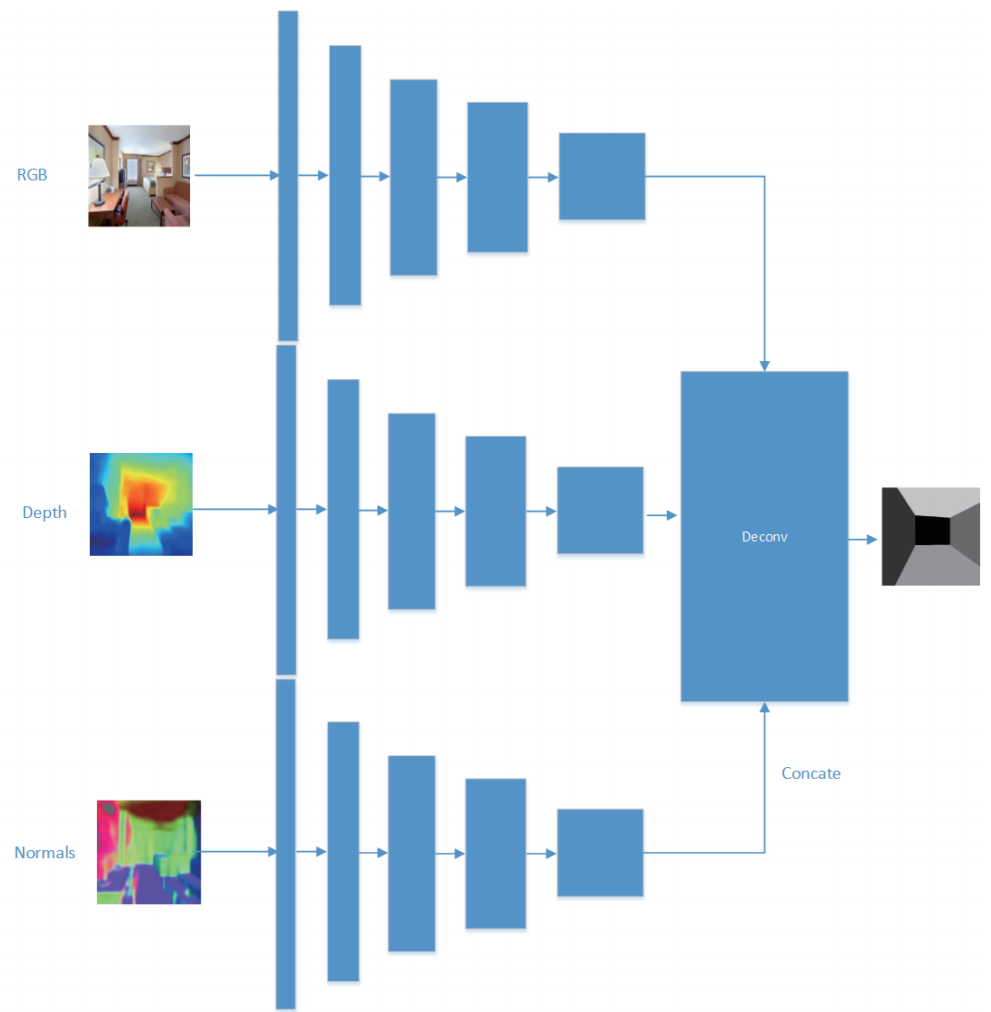
\includegraphics[width=\columnwidth]{figure/fcn-geometric-fusion.png}
	\caption{A network architecture that fuses the RGB, depth and normal together later. \cxj{add more details of each layer.}}
	\label{fig:fcn-geometric-fusion}
\end{figure}


For both networks to predict the five surface maps, the loss function is defined as the softmax ...\cxj{check wiht Fengjuntao. thesis page 18.}
\cxj{The output is five maps or a single map with five surface labels?}


\textbf{Training}
\cxj{How do you train this network with additional input? Any option to change the network? Do you modified the network parameters? say number of neurons or layers?}

\begin{figure}[!htq]
	\centering 
	\textsc{\includegraphics[width=3.4in]{figure/fcn.eps}}
	\caption{Layout estimation results using different architectures. Row from top to bottom: (a) the input RGB image. (b)(c)(d)Surface predictions using the FCNN architecture used in \cite{dasgupta2016delay,ren2016coarse}, our FCN-MC and FCN-GF respectively. (e) The ground truth. }
	\label{fig:fcn-comparison}
\end{figure}

\cxj{Result analysis for different architures. } 
From Table~\ref{table:fcn-accuracy}, we can see that ...\cxj{FCN-GF is better than FCN-MC?}
Our method generate much more clear edges, less holes. 


\begin{table}
	\centering
	\caption{Pixelwise accuracy for surface label prediction.}
	\label{table:fcn-accuracy}
	\begin{tabular}{c|c}
		\hline
	Network & Accuracy\\
	\hline
	FCN-32s & 0.8109 \\ 
	FCN-MC  & 0.8392 \\
	FCN-GF  & 0.8350 \\
		\hline
	\end{tabular}
		
\end{table}



\cxj{Do test on RGBD images...}




\subsection{Layout Generation}
\label{subsection:optimization}
We adopt a popular model that several  researchers~\cite{hedau2009recovering,dasgupta2016delay,ren2016coarse} have been used to parameterize indoor layout based on the Manhattan world assumption. 
Indoor scene layout can be modeled as 

\begin{equation}
	\label{eq:Layout}
	L = (l1, l2, l3, l4, v)
\end{equation}
where $l_{i}$ stands for $i^{th}$ vanishing line and $v$ stands for the specific vanishing point. The whole scene is equivalent to be labeled to five semantic surfaces, coresponding to (front, left, right, ceiling, ground), as described in Fig. \ref{fig:2.model}. Based ob Eq. (\ref{1.Layout}), each surface can be reconstructed with vanishing lines, extension lines between vanishing point and Intersection point, and image boundaries. Due to the camera pose, not five surfaces are always visible, and such layout can still be modeled by Eq. (\ref{1.Layout}). Different examples are given in Fig. \ref{fig:3.example}.